% Тип документа
\documentclass[a4paper,12pt]{extarticle}

% Шрифты, кодировки, символьные таблицы, переносы
\usepackage{cmap}
\usepackage[T2A]{fontenc}
\usepackage[utf8x]{inputenc}
\usepackage[russian]{babel}

% Это пакет -- хитрый пакет, он нужен но не нужен
\usepackage[mode=buildnew]{standalone}

\usepackage
	{
		% Дополнения Американского математического общества (AMS)
		amssymb,
		amsfonts,
		amsmath,
		amsthm,
		physics,
		% misccorr,
		% 
		% Графики и рисунки
		wrapfig,
		graphicx,
		subcaption,
		float,
		tikz,
		tikz-3dplot,
		caption,
		csvsimple,
		color,
		booktabs,
		pgfplots,
		pgfplotstable,
		geometry,
		% 
		% Таблицы, списки
		makecell,
		multirow,
		indentfirst,
		%
		% Интегралы и прочие обозначения
		ulem,
		esint,
		esdiff,
		% 
		% Колонтитулы
		fancyhdr,
	}  

\usepackage{xcolor}
\usepackage{hyperref}

 % Цвета для гиперссылок
\definecolor{linkcolor}{HTML}{000000} % цвет ссылок
\definecolor{urlcolor}{HTML}{799B03} % цвет гиперссылок
 
\hypersetup{pdfstartview=FitH,  linkcolor=linkcolor,urlcolor=urlcolor, colorlinks=true}
% Обводка текста в TikZ
\usepackage[outline]{contour}

% Увеличенный межстрочный интервал, французские пробелы
\linespread{1.3} 
\frenchspacing 

 
\usetikzlibrary
	{
		decorations.pathreplacing,
		decorations.pathmorphing,
		patterns,
		calc,
		scopes,
		arrows,
		fadings,
		through,
		shapes.misc,
		arrows.meta,
		3d,
		quotes,
		angles,
		babel
	}


\tikzset{
	force/.style=	{
		>=latex,
		draw=blue,
		fill=blue,
				 	}, 
	%				 	
	axis/.style=	{
		densely dashed,
		blue,
		line width=1pt,
		font=\small,
					},
	%
	th/.style=	{
		line width=1pt},
	%
	acceleration/.style={
		>=open triangle 60,
		draw=magenta,
		fill=magenta,
					},
	%
	inforce/.style=	{
		force,
		double equal sign distance=2pt,
					},
	%
	interface/.style={
		pattern = north east lines, 
		draw    = none, 
		pattern color=gray!60,
					},
	cross/.style=	{
		cross out, 
		draw=black, 
		minimum size=2*(#1-\pgflinewidth), 
		inner sep=0pt, outer sep=0pt,
					},
	%
	cargo/.style=	{
		rectangle, 
		fill=black!70, 
		inner sep=2.5mm,
					},
	%
	caption/.style= {
		midway,
		fill=white!20, 
		opacity=0.9
					},
	%
	}

\newenvironment{tikzpict}
    {
	    \begin{figure}[htbp]
		\centering
		\begin{tikzpicture}
    }
    { 
		\end{tikzpicture}
		% \caption{caption}
		% \label{fig:label}
		\end{figure}
    }


\newcommand{\vbLabel}[3]{\draw ($(#1,#2)+(0,5pt)$) -- ($(#1,#2)-(0,5pt)$) node[below]{#3}}
\newcommand{\vaLabel}[3]{\draw ($(#1,#2)+(0,5pt)$) node[above]{#3} -- ($(#1,#2)-(0,5pt)$) }

\newcommand{\hrLabel}[3]{\draw ($(#1,#2)+(5pt,0)$) -- ($(#1,#2)-(5pt,0)$) node[right, xshift=1em]{#3}}
\newcommand{\hlLabel}[3]{\draw ($(#1,#2)+(5pt,0)$) node[left, xshift=-1em]{#3} -- ($(#1,#2)-(5pt,0)$) }



\newcommand\zi{^{\,*}_i}
\newcommand\sumn{\sum_{i=1}^{N}}

\tikzset{
	coordsys/.style={scale=1.8,x={(1.1cm,-0cm)},y={(0.5cm,1cm)}, z={(0cm,0.8cm)}},
	coordsys/.style={scale=1.5,x={(0cm,0cm)},y={(1cm,0cm)}, z={(0cm,1cm)}}, 
	coordsys/.style={scale=1.5,x={(1cm,0cm)},y={(0cm,1cm)}, z={(0cm,0cm)}}, 
}

\usepgfplotslibrary{units}


% Draw line annotation
% Input:
%   #1 Line offset (optional)
%   #2 Line angle
%   #3 Line length
%   #5 Line label
% Example:
%   \lineann[1]{30}{2}{$L_1$}

\newcommand{\lineann}[4][0.5]{%
    \begin{scope}[rotate=#2, blue,inner sep=2pt, ]
        \draw[dashed, blue!40] (0,0) -- +(0,#1)
            node [coordinate, near end] (a) {};
        \draw[dashed, blue!40] (#3,0) -- +(0,#1)
            node [coordinate, near end] (b) {};
        \draw[|<->|] (a) -- node[fill=white, scale=0.8] {#4} (b);
    \end{scope}
}

\newcommand{\lineannn}[4][0.5]{%
    \begin{scope}[rotate=#2, blue,inner sep=2pt, ]
        \draw[dashed, blue!40] (0,0) -- +(0,#1)
            node [coordinate, near end] (a) {};
        \draw[dashed, blue!40] (#3,0) -- +(0,#1)
            node [coordinate, near end] (b) {};
        % \draw[color=white, color=blue] (a) -- node[fill=white, scale=0.8] {#4} (b);
        \draw[->|] (a)++(-0.3,0) -- (a);
        \draw[->|] (b)++(0.3,0) coordinate (xx) -- (b);
        \draw (xx) node[fill=white, scale=0.8, right] {#4};
    \end{scope}
}

% Круговая стрелка относительно центра (дуга из центра)
\tikzset{
  pics/carc/.style args={#1:#2:#3}{
    code={
      \draw[pic actions] (#1:#3) arc(#1:#2:#3);
    }
  },
  dash/.style={
  	dash pattern=on 5mm off 5mm
  }
}

% Среднее <#1>
\newcommand{\mean}[1]{\langle#1\rangle}

\pgfplotsset{
    % most recent feature set of pgfplots
    compat=newest,
}

% const прямым шрифтом
\newcommand\ct[1]{\text{\rmfamily\upshape #1}}
\newcommand*{\const}{\ct{const}}


\usepackage[europeanresistors,americaninductors]{circuitikz}

% Style to select only points from #1 to #2 (inclusive)
\pgfplotsset{select/.style 2 args={
    x filter/.code={
        \ifnum\coordindex<#1\def\pgfmathresult{}\fi
        \ifnum\coordindex>#2\def\pgfmathresult{}\fi
    }
}}


\usepackage{array}
\usepackage{pstool}


%%%%%%%%%%%%%%%%%%%%%%%%%%%%%%%%%%%%%%%%%%%%%%%%%
\makeatletter
\newif\if@gather@prefix 
\preto\place@tag@gather{% 
  \if@gather@prefix\iftagsleft@ 
    \kern-\gdisplaywidth@ 
    \rlap{\gather@prefix}% 
    \kern\gdisplaywidth@ 
  \fi\fi 
} 
\appto\place@tag@gather{% 
  \if@gather@prefix\iftagsleft@\else 
    \kern-\displaywidth 
    \rlap{\gather@prefix}% 
    \kern\displaywidth 
  \fi\fi 
  \global\@gather@prefixfalse 
} 
\preto\place@tag{% 
  \if@gather@prefix\iftagsleft@ 
    \kern-\gdisplaywidth@ 
    \rlap{\gather@prefix}% 
    \kern\displaywidth@ 
  \fi\fi 
} 
\appto\place@tag{% 
  \if@gather@prefix\iftagsleft@\else 
    \kern-\displaywidth 
    \rlap{\gather@prefix}% 
    \kern\displaywidth 
  \fi\fi 
  \global\@gather@prefixfalse 
} 
\newcommand*{\beforetext}[1]{% 
  \ifmeasuring@\else
  \gdef\gather@prefix{#1}% 
  \global\@gather@prefixtrue 
  \fi
} 
\makeatother
%%%%%%%%%%%%%%%%%%%%%%%%%%%%%%%%%%%%%%%%%%%%%%%%%

\geometry		
	{
		left			=	2cm,
		right 			=	2cm,
		top 			=	3cm,
		bottom 			=	3cm,
		bindingoffset	=	0cm
	}

%%%%%%%%%%%%%%%%%%%%%%%%%%%%%%%%%%%%%%%%%%%%%%%%%%%%%%%%%%%%%%%%%%%%%%%%%%%%%%%



	%применим колонтитул к стилю страницы
\pagestyle{fancy} 
	%очистим "шапку" страницы
\fancyhead{} 
	%слева сверху на четных и справа на нечетных
\fancyhead[R]{\labauthors} 
	%справа сверху на четных и слева на нечетных
\fancyhead[L]{Отчёт по лабораторной работе №\labnumber} 
	%очистим "подвал" страницы
\fancyfoot{} 
	% номер страницы в нижнем колинтуле в центре
\fancyfoot[C]{\thepage} 

%%%%%%%%%%%%%%%%%%%%%%%%%%%%%%%%%%%%%%%%%%%%%%%%%%%%%%%%%%%%%%%%%%%%%%%%%%%%%%%

\renewcommand{\contentsname}{Оглавление}

\usepackage{tocloft}
% \renewcommand{\cftpartleader}{\cftdotfill{\cftdotsep}} % for parts
% \renewcommand{\cftsectiondotsep}{\cftdotsep}% Chapters should use dots in ToC
\renewcommand{\cftsecleader}{\cftdotfill{\cftdotsep}}
%\renewcommand{\cftsecleader}{\cftdotfill{\cftdotsep}} % for sections, if you really want! (It is default in report and book class (So you may not need it).
% ---------
% \newcommand{\cftchapaftersnum}{.}%
% \usepackage{titlesec}
% \titlelabel{\thetitle.\quad}
\usepackage{secdot}
\sectiondot{subsection}

\begin{document}

\def\labauthors{Войтович Д.А., Карусевич А.А., Разова А.А.}
\def\labgroup{430}
\def\labnumber{5}
\def\labtheme{Апериодический усилитель}
\renewcommand{\vec}{\mathbf}
\renewcommand{\Re}{\operatorname{Re}}
\renewcommand{\Im}{\operatorname{Im}}
\renewcommand{\phi}{\varphi}
\renewcommand{\hat}{\widehat}

\begin{titlepage}

\begin{center}

{\small\textsc{Нижегородский государственный университет имени Н.\,И. Лобачевского}}
\vskip 1pt \hrule \vskip 3pt
{\small\textsc{Радиофизический факультет}}

\vfill

{\Large Отчет по лабораторной работе №\labnumber\vskip 12pt\bfseries \labtheme}
	
\end{center}

\vfill
	
\begin{flushright}
	{Выполнили студенты \labgroup\ группы\\ \labauthors}%\vskip 12pt Принял:\\ Менсов С.\,Н.}
\end{flushright}
	
\vfill
	
\begin{center}
	Нижний Новгород, \the\year
\end{center}

\end{titlepage}



%\tableofcontents
\newpage

\section{Теоретическая часть}
\subsection{Цель работы}
Исследование транзисторных апериодических усилителей с общим эмиттером (ОЭ) и общим коллектором (ОК).

\subsection{Назначение устройства}
Основным назначением усилителя является увеличение мощности электрических колебаний без изменения их формы. Кроме того, усилитель часто используется для развязки каскадов или их согласования.

\subsection{Область использования}
Усилители электрических колебаний имеют широкое и разнообразное применение: в радиосвязи и радиовещании, телевидении, звуковом кино, устройствах записи и воспроизведения звука, дальней проводной связи, измерительной аппаратуре, а также в телемеханике, автоматике, электронно-вычислительных машинах, аппаратуре исследования космического пространства и т.д.

\subsection{\textbf{Принципы работы усилителя}}
Качественные показатели усилителя во многом определяются режимом его работы. Под режимом работы понимается совокупность токов и напряжений в схеме, определяющих положение «точки покоя», т.е. состояние схемы до подачи на ее вход управляющего (входного) колебания.

При работе с сильными сигналами (обычно это при $U_{\text{вх}}>10$мВ) выбирают ту область статических характеристик транзистора, которая обеспечивает получение заданной максимальной амплитуды тока, напряжения или мощности при допустимой величине
нелинейных искажений и, по возможности, небольшом расходе энергии источника питания. Этим требованиям и должен подчиняться выбор режима работы. Выбор несколько различается в зависимости от того, какой эффект на выходе усилителя желательно получить, и в зависимости от типа усиливаемых сигналов.

Если необходимо обеспечить заданную амплитуду выходного тока $I_m$ в низкоомной нагрузке, то режим выбирают следующим образом. Тип используемого транзистора выбирается с таким расчетом, чтобы его максимально допустимая величина коллекторного тока удовлетворяла условию $i_km\geqslant 2I_m$ при симметричных биполярных сигналах и $i_km>I_m$ при однополярных сигналах.

\begin{figure}[h]
	\centering
	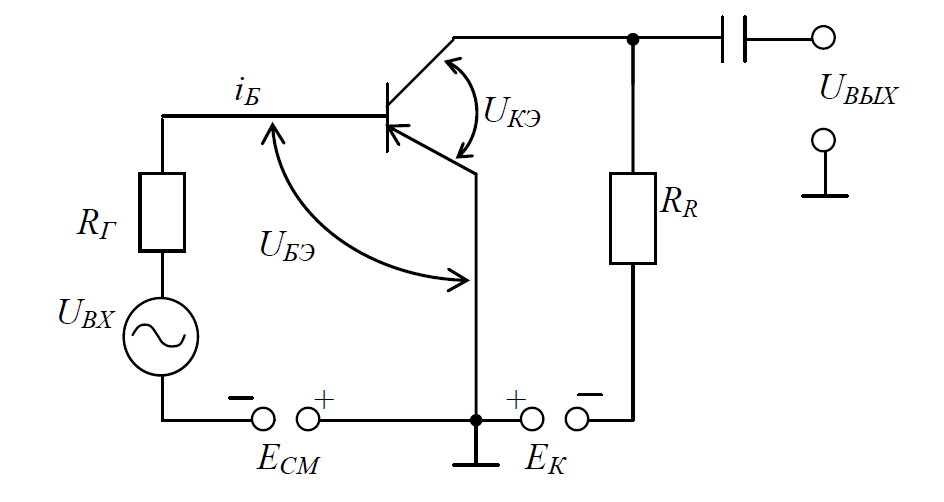
\includegraphics[width=0.5\linewidth]{fig/fig1}
	\caption{}
	\label{fig:1}
\end{figure}

В данной работе выбран транзистор МП41А.

\subsection{\textbf{Усилитель с общим эмиттером}}
В усилительных устройствах наиболее часто транзистор используется в схеме с общим эмиттером (ОЭ). В этой схеме (Рис.\ref{fig:1}) входным током является ток базы. Постоянная оставляющая тока базы задается величиной напряжения смещения $E_{\text{Б}}$, переменная составляющая создается источником сигнала $U_{\text{ВХ}}$ с внутренним сопротивлением $R_{\text{Г}}$. Выходным током называют ток коллектора. В его составе содержатся постоянная составляющая, определяемая начальным током базы и напряжением источника питания $E_{\text{К}}$, и переменная составляющая, пропорциональная управляющему напряжению $U_{\text{ВХ}}$. В реальной схемотехнике используются схемы усилителей, отличающиеся от схемы рис.\ref{fig:1} по ряду признаков. Рассмотрим простейшую из них (Рис.\ref{fig:2}):

\begin{figure}[h]
	\centering
	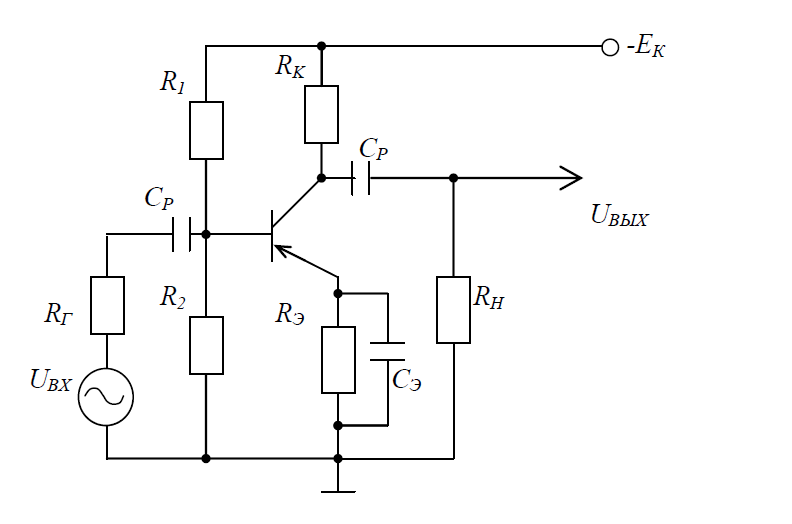
\includegraphics[width=0.5\linewidth]{fig/fig2}
	\caption{}
	\label{fig:2}
\end{figure}

Во-первых, в этой схеме отсутствует источник смещения $E_{\text{СМ}}$. Необходимое напряжение смещений создается за счет делителя напряжения $R_1$ и $R_2$, который, с учетом напряжения на резисторе $R_{\text{Э}}$, обеспечивает требуемое по величине и знаку постоянное напряжение на переходе база – эмиттер, и, следовательно, требуемое значение постоянной составляющей тока базы.

Во-вторых, в схему включены разделительные конденсаторы $C_p$, предназначенные для устранения влияния источника сигнала и внешней нагрузки $R_H$ на режим работы каскада. Конденсатор $C_p$ на входе совместно с входным сопротивлением каскада образует частотно – зависимый делитель, который уменьшает общий коэффициент усиления усилителя на нижних частотах. Аналогично учитывается влияние делителя $C_p$ и $R_H$. 

В-третьих, в схему включена цепочка $R_{\text{Э}}$ $C_{\text{Э}}$, предназначенная для температурной стабилизации режима  усилителя. Дело в том, что с повышением температуры окружающей среды в транзисторах наблюдается тепловой сдвиг вольт – амперных характеристик и, как следствие, изменение режима усилителя. Для снижения отрицательных последствий теплового сдвига в транзисторных усилителях реализуется термостабилизация режима. В ее основу положен механизм отрицательной обратной связи.

Термостабилизирующую роль $R_{\text{Э}}$, как элемента отрицательной связи можно описать на качественном уровне следующим образом. Пусть при начальной температуре среды ток базы равен $i_{\text{Б0}}$, напряжение смещения $U_{\text{Б0}}$, постоянная составляющая тока коллектора $i_{\text{K0}}$. С ростом температуры происходит тепловой сдвиг характеристик, в результате чего коллекторный ток получит приращение $\Delta i_{Kn}$. Это вызовет приращение напряжения на $R_{\text{Э}}$, равное $\Delta i_{Kn}R_{\text{Э}}$ . На эту же величину изменится смещение $U_{\text{Б0}}-\Delta i_{Kn}R_{\text{Э}}$, что приведет к уменьшению тока базы и к соответствующему уменьшению тока коллектора. Рабочая точка будет смещена к исходному положению, т.е. стабилизирована. Если емкость $C_{\text{Э}}$ отсутствует, то отрицательная обратная связь через $R_{\text{Э}}$ приведет к снижению усиления каскада. Чтобы избежать этого, сопротивление $R_{\text{Э}}$ шунтируют большой емкостью $C_{\text{Э}}$, что сохраняет отрицательную обратную связь только по постоянному току.

Рассмотрим работу усилителя. На рис.\ref{fig:3} приведены осциллограммы действующих в усилителе токов и напряжений, иллюстрирующие процессы, происходящие в схеме. На рис.3а представлено, взятое из справочника по транзисторам, семейство выходных статических характеристик. На этом же рисунке изображена нагрузочная прямая, исходящая из точки (0,-10) под углом $\alpha$; $tg\alpha = \frac{1}{R_K}$. Входная динамическая характеристика транзистора (рис.3б) практически совпадает со статической входной характеристикой, снятой при $U_{\text{КЭ}}$=-5В. Это объясняется слабым влиянием коллекторного напряжения на ток базы.

Напряжение на базе $U_{\text{БЭ}}$=-0.225В и ток базы $I_{\text{БП}}$=0.2мА
определяют режим транзистора по постоянному току (“точка покоя” на нагрузочной прямой: $I_{\text{Кn}}$=0.2мА, $U_{\text{КЭn}}$= -4.5В).

Изменение входного напряжения (под действием сигнала) вызывает изменение тока базы. При изменении тока базы изменяется ток коллектора и в коллекторной цепи выделяется
усиленный сигнал, который через разделительный конденсатор $C_P$ поступает на выход усилителя. Для данной схемы

входное сопротивление $R_{\text{ВХ}}=\frac{\Delta U_{\text{БЭ}}}{\Delta I_{\text{БЭ}}}=\frac{0.035}{0.1\cdot10^{-3}}=350 \text{ Ом},$

коэффициент передачи по току $K_i=\frac{\Delta I_K}{\Delta I_{\text{Б}}}=\frac{6.5}{0.1}=65,$

по напряжению $K_U=\frac{\Delta U_{\text{KЭ}}}{\Delta U_{\text{БЭ}}}=\frac{2.5}{0.035}=71.5,$

и по мощности $K_P=K_i K_U=6.5\cdot 71.5=4650$

Таким образом, мощность, выделяемая на сопротивлении нагрузки $R_K$ переменной составляющей коллекторного тока, значительно больше мощности входного сигнала, затрачиваемой во входной цепи усилителя.

\begin{figure}[h]
	\centering
	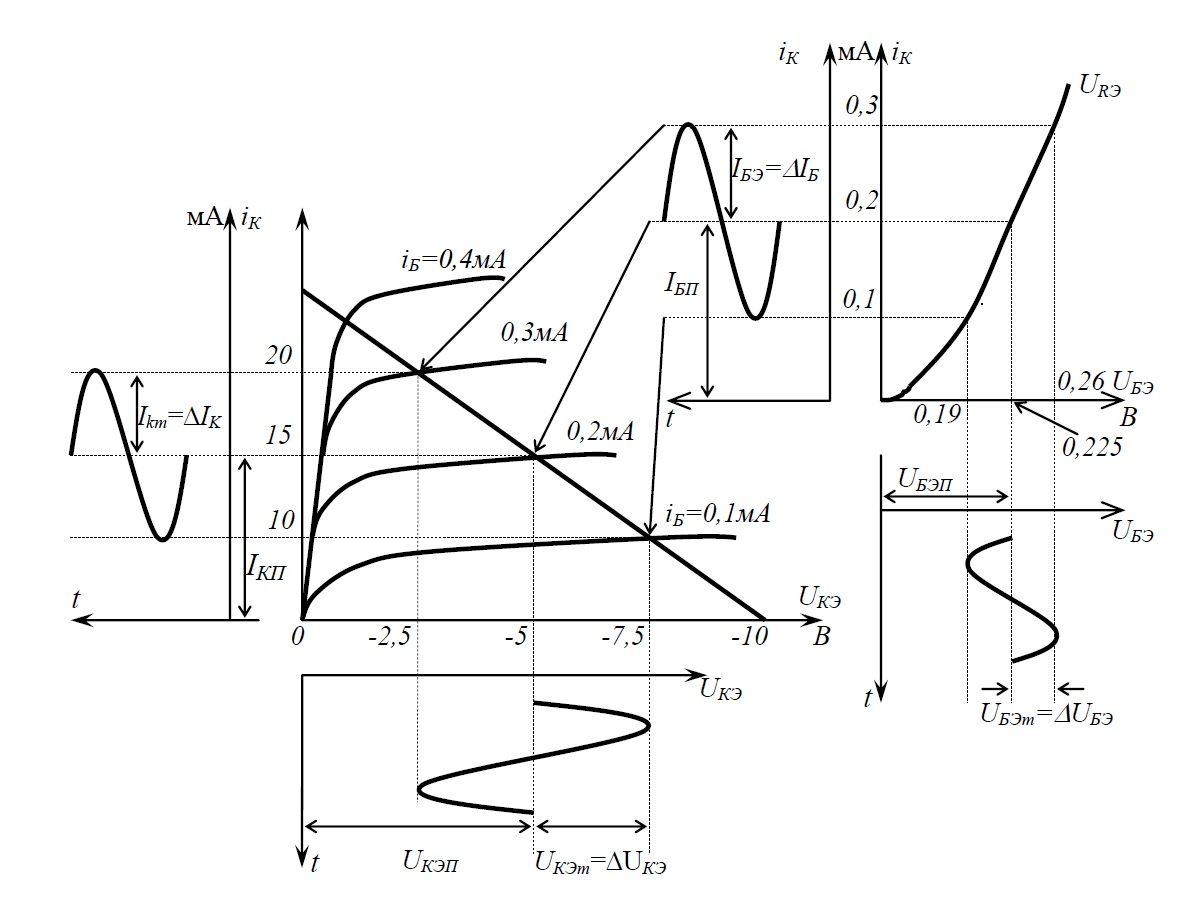
\includegraphics[width=\linewidth]{fig/fig3}
	\caption{}
	\label{fig:3}
\end{figure}

С практической точки зрения важно исследовать частотные свойства усилителя, которые исчерпывающим образом описываются комплексным коэффициентом передачи $K(j\omega)$. При вычислении $K(j\omega)$ усилителя приходится считаться со следующим обстоятельством. Схемы рис.\ref{fig:2} и \ref{fig:4} являются принципиальными схемами. Такие схемы, содержащие активные элементы (диоды, транзисторы и др.) удобны при описании принципа действия каскадов, однако к ним не приемлемы известные математические методы описания электрических цепей. По этой причине широко используются схемы замещения или эквивалентные схемы.

\subsection{\textbf{Частотные свойства каскада с общим эмиттером}}
Электронный усилитель в своем составе имеет 

1)усилительный прибор (транзистор в рассматриваемом случае)
2)соответствующую рабочему диапазону частот нагрузку в его
выходной цепи.

Режим работы усилительного прибора по постоянному току обеспечивается двумя источниками напряжения. Один питает коллекторную цепь транзистора, второй создает
напряжение смещения $Е_{\text{см}}$ на базе. Чаще всего используется один источник напряжения питания Е. В таких случаях $Е_{\text{см}}$ получают, применяя делитель напряжения на сопротивлениях. Именно такая усилительная секция представлена на рис. 1а. В ней коллекторной нагрузкой транзистора является резистор $R_k$, потенциал базы
задается делителем напряжения $R_1-R_2$, а резистор $R_{\text{Э}}$ в цепи эмиттера служит для температурной стабилизации параметров транзистора Т. Емкости $С_1$ и $С_2$ являются разделительными и предназначены для того, чтобы источник сигнала и внешняя нагрузка (импеданс внешней нагрузки равен $Z_{ВН}$) не влияли на режим транзистора по постоянному току. Но эти емкости не должны влиять и на прохождение сигнала в полосе пропускания усилителя. Поэтому их величины выбираются такими, чтобы во всей полосе пропускания усилителя импедансы емкостей $С_1$ и $С_2$ были незначительны и выполнялись неравенства

\begin{equation}
	\frac{1}{\omega C_1}\ll R_{\text{ВХ}}, \frac{1}{\omega C_2}\ll |Z_{\text{ВХ}}|.
	\label{eq:1}
\end{equation}

В \ref{eq:1} $R_{\text{ВХ}}$ представляет входное сопротивление каскада. Оно образовано параллельно включенными резисторами $R_1$ и $R_2$ и входным  сопротивлением транзистора $R_{\text{ВХ.ТР}}$:

$$R_{\text{ВХ}}=(R_1||R_2||R_{\text{ВХ.ТР}}).$$

\begin{figure}[h]
	\centering
	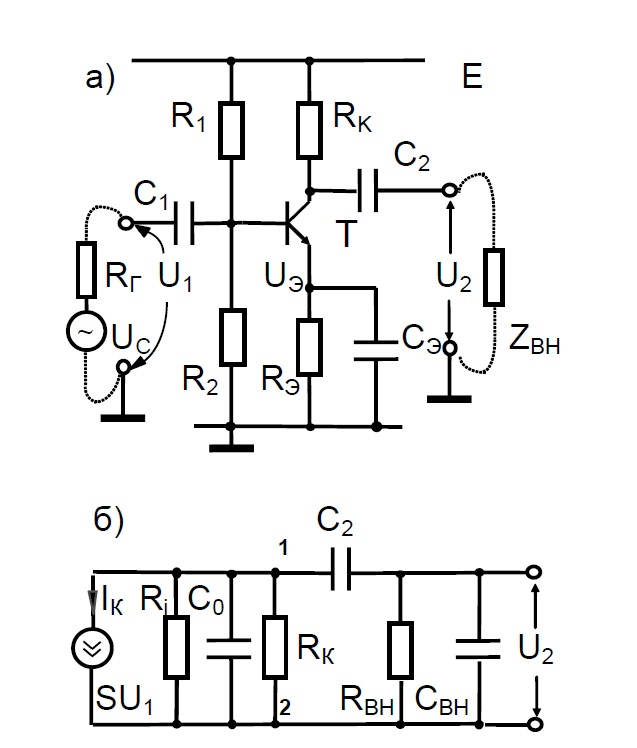
\includegraphics[width=0.6\linewidth]{fig/fig4}
	\caption{}
	\label{fig:4}
\end{figure}

Среди трех названных составляющих $R_{\text{ВХ}}$ наименьшую величину имеет входное сопротивление транзистора, которое равно объемному сопротивлению базы $r_{\text{б}}\approx 300\text{Ом}$. При столь малом входном сопротивлении ($R_{\text{ВХ}}<r_{\text{б}}$), емкость $C_1$ должна быть достаточно большой, чтобы не было ее влияния на частотные свойства усилителя, особенно в области низких частот. Достаточно большой выбирается и емкость $C_{\text{Э}}$, поскольку она обеспечивает “заземление” общего электрода - эмиттера по переменному току:

\begin{equation}
	\frac{1}{\omega C_{\text{Э}}}\ll R_{\text{Э}}.
	\label{eq:2}
\end{equation}

Назначение емкости $C_{\text{Э}}$ состоит в том, что она снимает отрицательную обратную связь по переменному току через сопротивление $R_{\text{Э}}$. Такая связь возникает при отсутствии $C_{\text{Э}}$.

Найдем коэффициент передачи и его зависимость от частоты - амплитудно-частотную характеристику (АЧХ) - изображенного на рис.4а усилительного каскада. Для этого составим эквивалентную схему каскада по переменному току. Такая схема - это модель усилителя, которая включает лишь существенные для процесса усиления компоненты. Конкретный вид эквивалентной схемы зависит от многих факторов. Среди них, в частности, уровень входного сигнала, питающие транзистор постоянные токи и
напряжения, рабочий диапазон частот и требуемая выходная мощность. Рассматриваемый нами усилитель (рис.4а) является усилителем напряжения. В этом случае применимо малосигнальное приближение, при котором допускается, что вызываемые входным
сигналом приращения токов и напряжений не изменяют дифференциальных параметров транзистора - коэффициента усиления тока базы $\beta$, входного сопротивления $R_{\text{ВХ.ТР}}$ и внутреннего сопротивления $R_i$ (сопротивления между коллектором и эмиттером). Их можно считать постоянными и не зависящими от входного сигнала. В таком случае транзистор работает как управляемый током базы источник тока с внутренним сопротивлением $R_i$:

$$\Delta i_k = \beta \cdot \Delta i_{\text{б}}.$$

Здесь $i_k$ и $i_{\text{б}}$ - соответственно приращения токов коллектора и базы транзистора. Элементы цепей питания в явном виде в эквивалентную схему могут не войти. Это зависит от того, являются ли эти элементы значимыми для переменных, обусловленных входным сигналом токов или нет. К таким элементам относятся резисторы $R_1$, $R_2$ и $R_{\text{Э}}$. Как уже отмечалось, резисторы $R_1$ и $R_2$ задают напряжение смещения на базу транзистора, а $R_{\text{Э}}$ обеспечивает температурную стабилизацию его параметров за счет отрицательной обратной связи по постоянному току. Цепи питания определяют конкретные, ими задаваемые значения дифференциальных параметров транзистора $\beta$, $R_{\text{ВХ.ТР}}$ и $R_i$.

Если ко входу усилительной секции подключен источник напряжения $U_C$, у которого внутреннее сопротивление (сопротивление генератора $R_{\text{Г}}$) много меньше входного сопротивления $R_{\text{ВХ}}$, допустимо представление транзистора источником тока, управляемым напряжением. В этом случае

$$\Delta i_k = S\cdot \Delta u_{\text{бэ}},$$
$u_{\text{бэ}}$- приращение разности потенциалов между базой и эмиттером, а $S=\beta/R_{\text{ВХ}} \approx \beta/r_{\text{б}}$ - крутизна транзистора. Если сигнал на входе
синусоидален, то все напряжения $u$ и токи $i$ можно представить
комплексными амплитудами $U=|U|\cdot \exp(j\varphi_u)$ и $I=|I|\cdot \exp(\varphi_i)$, где |U| и |I| - амплитуды, а $\varphi_u$ и $\varphi_i$ - фазы соответствующих напряжений и токов. Переменная составляющая управляющего напряжения (напряжения на базе $U_{\text{БЭ}}$) отличается от напряжения сигнала $U_C$.Однако при $R_{\text{Г}}\ll R_{\text{ВХ}},\frac{1}{\omega C_1}\ll R_{\text{ВХ}}$ и $\frac{1}{\omega C_{\text{Э}}}\ll R_{\text{Э}}$~~$U_{\text{Б}} \approx U_1 \approx U_C$ то есть переменная составляющая управляющего напряжения равна входному сигналу, который, в свою очередь, равен напряжению источника сигнала.

В общем случае эквивалентная схема усилителя содержит входную (базовую) и выходную (коллекторную) цепи, а также элементы их взаимосвязи. Связь между входной и выходной цепями, называемая обратной, возникает из-за емкости коллектор-база $C_{\text{КБ}}$ и из-за конечной величины сопротивления $r_{\text{Э}}$ эмиттерного перехода транзистора. Первая является обратной связью по напряжению, вторая - по току. Обратная связь через $C_{\text{КБ}}$ не существенна в области низких частот, то есть в той частотной области, на которую рассчитан рассматриваемый усилитель. Обратную связь через $r_{\text{Э}}$ можно не учитывать, если величина импеданса в цепи эмиттера $|Z_{\text{Э}}|=| (R_{\text{Э}}||C_{\text{Э}})|\gg r_{\text{Э}}$. При выполнении перечисленных выше условий входную и выходную цепи усилительной секции можно рассматривать независимо. Будем полагать также, что во входной цепи выполнены условия согласования по напряжению с источником сигнала, то есть $R_{\text{Г}} \ll R_{\text{ВХ}}$, а разделительная емкость $C_1$ такова, что ее импеданс $\frac{1}{\omega C_1} \ll R_{\text{ВХ}}$. В таком случае управляющее напряжение $U_{\text{Б}}$ равно входному $U_1$.

Эквивалентная схема выходной цепи усилителя приведена на рис. 4б. В ней транзистор Т представлен источником тока $S\cdot U_1$ c внутренним сопротивлением $R_i$ и выходной емкостью $C_0$. Последняя в значительной степени зависит от барьерной емкости коллекторного перехода транзистора. В эквивалентную схему вошли также выходная разделительная емкость $C_2$, коллекторная нагрузка транзистора $R_K$ и элементы, характеризующие внешнюю нагрузку усилителя $Z_{BH}$. Будем полагать, что внешняя нагрузка имеет емкостной характер и состоит из активного сопротивления $R_{BH}$ и емкости $C_{BH}$ ($Z_{BH}=(R_{BH}||C_{BH})$). Для начала положим $C_{BH}=0$. Тогда коэффициент передачи усилителя

$$K(j\omega)=\frac{U_2}{U_1}=\frac{U_{12}}{U_1} \cdot \frac{U_2}{\frac{U_2}{U_1}}$$
где $U_{12}$ - разность потенциалов между точками 1 и 2 в схеме на рис.1б. Выражая $U_2$ и $U_{12}$ через действующие в схеме токи получим

$$K(j\omega)=-\frac{SU_1}{\{\frac{1}{R_i}+j\omega C_0+\frac{1}{R_K}+(R_{BH}+\frac{1}{i\omega C_2})^{-1}\}U_1} \cdot \frac{U_{12}R_{BH}}{(R_{BH}+\frac{1}{i\omega C_2})U_{12}}$$

Обозначим через $R_{\sum}=(R_i||R_K||R_{BH})$ результирующее сопротивление параллельно включенных резисторов $R_i$, $R_K$ и $R_{BH}$. Среди них $R_i$ имеет наибольшую величину ($\sim$ нескольких сотен кОм) и поэтому $R_{\sum} \approx (R_K||R_{BH})$. Введем также постоянные времени $\tau_1=C_2 R_{BH}$ и $\tau_2=C_0 R_{\sum}$ и коэффициент $\gamma=(R_K||R_i)\geq 1$. Кроме того, учтем то, что в реальных усилителях обычно $C_0 \ll C_1,C_2$. В итоге получим для коэффициента передачи выражение

\begin{equation}
	K(j\omega) \approx \frac{-SR_{\sum}}{1-j(\frac{1}{\gamma \omega \tau_1}-\omega \tau_2)}=|K(j \omega)| \cdot \exp(j \varphi(\omega))
	\label{eq:3}
\end{equation}

По смыслу $\tau_1$ - это постоянная времени цепи, образованной разделительным конденсатором $C_2$ и сопротивлением внешней нагрузки, а $\tau_2$ - постоянная времени цепи, состоящей из выходной емкости транзистора $C_0$ и включенных параллельно ей  резисторов $R_i$, $R_K$ и $R_{BH}$.

\begin{figure}[h!]
	\centering
	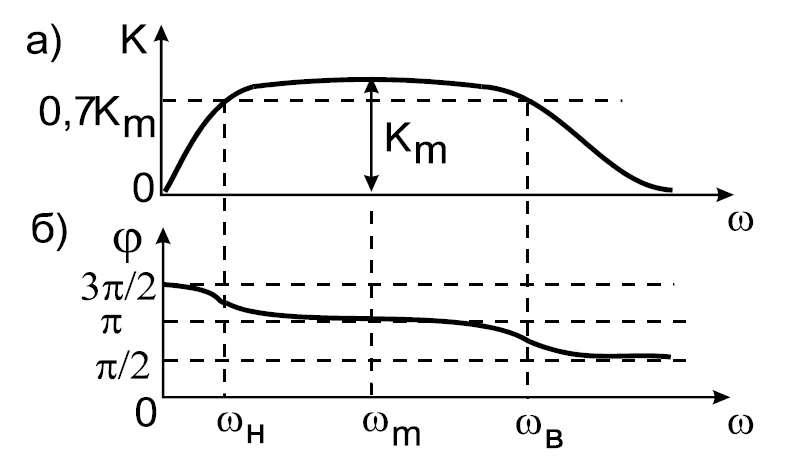
\includegraphics[width=0.6\linewidth]{fig/fig5}
	\caption{}
	\label{fig:5}
\end{figure}

Полученный из (\ref{eq:3}) графический вид амплитудно-частотной (АЧХ) и фазо-частотной (ФЧХ) характеристик, качественно изображен на рис.\ref{fig:5}. На рис.5а представлена зависимость модуля коэффициента передачи $K(\omega) = |K(j\omega)|$, а на рис. 5б - зависимость аргумента $\varphi(\omega)$ от частоты. Можно выделить три характерные
частотные области этих характеристик:

1)средняя область между нижней $\omega_H$ и верхней $\omega_B$ частотами, где коэффициент передачи почти постоянен. Разность между $\omega_B$ и $\omega_H$ определяет полосу пропускания усилителя $\text{П}=\omega_B - \omega_H$. Значения $\omega_H$ и верхней $\omega_B$ вычисляются по задаваемому уменьшению модуля коэффициента передачи по отношению к его максимальному значению $K_m=K(\omega_m)$, достигаемому при $\omega=\omega_m=\frac{1}{\gamma \tau_1 \tau_2}$. Для коэффициента передачи по напряжению принято вычислять граничные частоты полосы пропускания по уровню $\frac{1}{\sqrt{2}} \approx 0.7$ от максимального значения $K_m$. В пределах полосы пропускания $K(\omega) \approx K_m \approx SR_{\sum}$. Выходная емкость транзистора $C_0$ и разделительная емкость $C_2$ здесь не оказывают существенного влияния; 

2)область низких частот ($0 <\omega<\omega_H$), где $K(\omega)$ уменьшается по мере приближения к нулевой частоте. Причина этого уменьшения обусловлена разделительной емкостью $C_2$, импеданс которой увеличивается при $\omega \rightarrow 0$. Заметим, что в этой области существенным может оказаться и влияние емкости в цепи эмиттера $C_{\text{Э}}$. Если ее импеданс $1/C_{\text{Э}}$ окажется сравнимым с величиной $R_{\text{Э}}$, то возникает отрицательная обратная связь по току, ведущая к уменьшению коэффициента передачи. Поэтому $C_{\text{Э}}$ должна быть достаточно большой, чтобы условие отсутствия обратной связи через эмиттерную цепь выполнялось во всей области усиливаемых частот. Для очень низких значений $\omega_H$ технически это требование трудно выполнить, поскольку величина $R_{\text{Э}}$, как правило, не велика (порядка 100 Ом);

3)область верхних частот ($\omega > \omega_B$). Здесь $К(\omega)$ уменьшается с ростом $\omega$ из-за уменьшения импеданса емкости $C_0$, которая включена параллельно результирующей нагрузке $R_{\sum}$ по переменному току.

Нужно сказать, что при $C_0\ll C_2~~~\tau_2 \ll \tau_1$ и емкости $C_0$ и $C_2$ оказывают воздействие на достаточно разнесенные по частоте области АЧХ с $\omega<\omega_H$ и $\omega>\omega_B$. Между ними находится достаточно протяженная полоса пропускания с почти постоянным коэффициентом усиления. Таким образом, в соответствии с принятой моделью $К_m$ не зависит ни от $C_0$, ни от $C_2$, а определяется только результирующей активной нагрузкой $R_{\sum}$. 

Фазовая характеристика усилителя $\varphi(\omega)$ (рис. 5б) связана с его АЧХ. Можно заметить, что там, где $К(\omega) \approx const$, ФЧХ линейна. Там же, где АЧХ изменяется, ФЧХ становится нелинейной. В полосе пропускания $\varphi(\omega) \approx \pi$. Это значит, что при $\omega \approx \omega_m$ фаза выходного сигнала по знаку противоположна фазе входного. Для сигнала с шириной спектра, не выходящей за пределы полосы пропускания П, усилительный каскад с общим эмиттером является фазоинвертирующим.

Если внешняя нагрузка усилителя помимо резистора $R_{BH}$ имеет еще и емкость $C_{BH}$, то верхняя граничная частота полосы пропускания $\omega_B$ понизится. Для достаточно малых $C_{BH}<<C_2$ изменение $\omega_B$ находится достаточно просто: в эквивалентной схеме по переменному току (рис.4б) параллельно емкости $C_0$ нужно подключить $C_{BH}$, а во входящей в выражение (\ref{eq:3}) постоянной времени $\tau_2$ вместо емкости $C_0$ взять суммарную емкость параллельно включенных $C_0$ и $C_{BH}$ (взять $\tau_2 = R_{\sum}(C_0||C_{BH})$).

Рассмотрим, наконец, входную (базовую) цепь усилителя. Она состоит из разделительной емкости $C_1$, параллельно включенных по переменному току резисторов $R_1$ и $R_2$, к которым подключено также входное сопротивление транзистора $R_{\text{ВХ.ТР}}$. По своему виду эта цепь аналогична выходной разделительной RC-цепи, состоящей из выходной разделительной емкости $C_2$ и внешней нагрузки $R_{BH}$. Разница в том, что вместо емкости $C_2$ на входе стоит емкость $C_1$, а вместо сопротивления $R_{BH}$ - входное сопротивление усилителя $R_{BH}= (R_1||R_2||R_{BH})$. На низких частотах входная разделительная RC- цепь может вызвать дополнительное уменьшение сигнала на базе
транзистора и, следовательно, нежелательное повышение нижней граничной частоты $\omega_H$, что сузит полосу пропускания П усилительного каскада.

\subsection{\textbf{Каскад по схеме с общим коллектором эмиттерный повторитель}}
Как видно из (\ref{eq:3}), величина коэффициента усиления каскада с общим эмиттером зависит не только от входящих в него элементов, но и от параметров подключаемой к выходу каскада нагрузки. Чтобы избежать такого влияния приходится между усилительной секцией и ее нагрузкой включать согласующие цепи, в том числе и активные. Вариантом активной согласующей цепи является каскад с транзистором, включенным по схеме с общим коллектором - эмиттерный повторитель (рис.6а). Как и в рассмотренной выше схеме с общим эмиттером, постоянный потенциал базы транзистора задается делителем напряжения на резисторах $R_1$ и $R_2$. Потенциал коллектора неизменен и равен напряжению источника питания Е. В отличие от схемы с общим эмиттером в эмиттерной цепи отсутствует емкость $C_{\text{Э}}$, Поэтому отрицательная обратная связь по току через $R_{\text{Э}}$ существенна не только для постоянной составляющей тока эмиттера, но и для его переменной составляющей. Сигнал на транзистор подается через разделительную емкость $C_1$, а снимается с нагрузки $R_{\text{Э}}$ в цепи эмиттера. При этом управляющее напряжение $U_{\text{УПР}}$ образуется как разность между напряжением на базе $U_{\text{Б}}$ и выходным напряжением транзистора (напряжением на эмиттере) $U_{\text{Э}}$:

\begin{equation}
	U_{\text{УПР}}=U_{\text{БЭ}}=U_{\text{Б}}-U_{\text{Э}}
	\label{eq:4}
\end{equation}

Соответствующая такому случаю эквивалентная схема выходной цепи транзистора по переменному току приведена на рис.6б. По-прежнему транзистор рассматривается как источник тока, управляемый напряжением. Его выходной ток - это ток эмиттера $I_{\text{Э}} \approx I_{\text{K}}=SU_{\text{УПР}}$, где $U_{\text{УПР}}$ определяется в соответствии с (\ref{eq:4}).

\begin{figure}[h!]
	\centering
	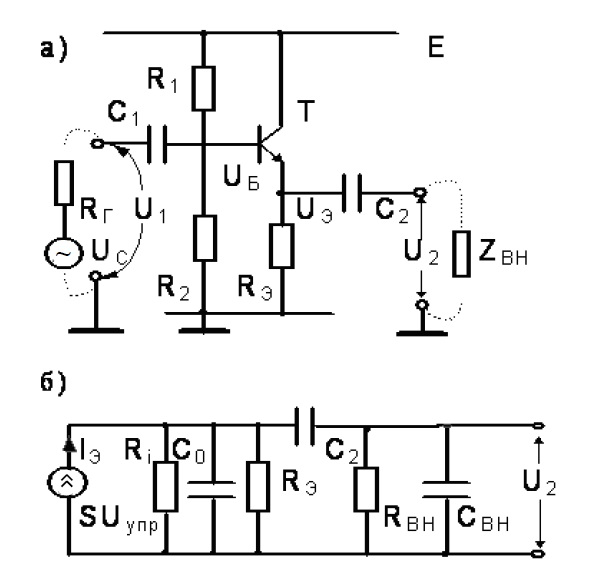
\includegraphics[width=0.6\linewidth]{fig/fig6}
	\caption{}
	\label{fig:6}
\end{figure}

В условиях согласования по напряжению, когда

$$R_{\text{Г}} \ll |Z_{\text{ВХ}}|=|U_1/I_1|$$
($U_1$ и $I_1$-соответственно входные напряжение и ток ), $U_1 \approx U_C$. Если
к тому же импеданс разделительной емкости $\frac{1}{\omega C_1}\ll R_{\text{ВХ.Б}}$- входного сопротивления в точке подключения базы транзистора, то напряжение на базе

\begin{equation}
	U_{\text{Б}} \approx U_1 \approx U_C
	\label{eq:5}
\end{equation}
и $Z_{\text{ВХ}} \approx R_{\text{ВХ}} \approx R_{\text{ВХ.Б}}$. Величина $R_{\text{ВХ.Б}}$ равна параллельно включенным сопротивлениям $R_1$, $R_2$ и $R_{\text{Б} \bot}$:

\begin{equation}
	R_{\text{ВХ.Б}}=(R_1||R_2||R_{\text{Б} \bot})
	\label{eq:6}
\end{equation}
где $R_{\text{Б} \bot}$ представляет сопротивление участка входной цепи, проходящего через эмиттерный переход транзистора. При выполнении условия (\ref{eq:3}) коэффициент передачи каскада с общим коллектором равен 

$$K=K(j\omega)=1=\frac{1}{SR_{\sum}}K,$$
откуда следует, что

$$K=\frac{1}{(1+\frac{1}{SR_{\sum}})}\leq 1.$$

Таким образом, усилитель, построенный по схеме с общим коллектором, не дает усиления по напряжению. Это есть следствие отрицательной обратной связи, при которой управляющее
напряжение образуется как разность между входным $U_1$ и выходным $U_2$ напряжениями. Обычно $SR_{\sum}\gg1$. Для обеспечения эффективной внешней обратной связи по току величина резистора $R_{\text{Э}}$ выбирается достаточно большой (по крайней мере $R_{\text{Э}} \gg r_{\text{Э}}$ - сопротивления эмиттерного перехода транзистора с характерным значением $\sim 10-15$ Ом), а $R_BH \sim R_{\text{Э}}$. Поэтому величина К близка к единице, что и обусловило название каскада эмиттерным повторителем. Основное назначение эмиттерного повторителя состоит в обеспечении условий согласования по напряжению при межкаскадных соединениях. Для этого требуется большое входное и малое выходное сопротивления. При выполнении (\ref{eq:5}) $R_{BX} \sim R_{\text{ВХ.Б}}$. Согласно (\ref{eq:6})  $R_{\text{ВХ.Б}}$ состоит из трех параллельно соединенных сопротивлений $R_1$, $R_2$ и $R_{\text{Б}}$.Последнее в схеме с общим коллектором имеет значительно большую величину, чем в схеме с общим эмиттером. Действительно,

$$R_{\text{Б} \bot}=\frac{U_{\text{Б}}}{I_{\text{Б}}} \approx \frac{U_2}{ \frac{ I_{ \text{Э} } }{\beta}}=\beta R_{\text{Э}}.$$

Поскольку $\beta \gg 1$, сопротивление  $R_{\text{ВХ.Б}} \approx R_{\text{Б} \bot}$ может быть весьма значительным. Выходное же сопротивление эмиттерного повторителя относительно невелико. Можно показать, что

$$R_{\text{ВЫХ}}=\frac{1}{S+\frac{1}{R_{\text{Э}}}} \approx \frac{1}{S}$$

Эти свойства эмиттерного повторителя дают возможность использования его в качестве согласующего каскада при работе на низкоомную внешнюю нагрузку.

\begin{figure}[h!]
	\centering
	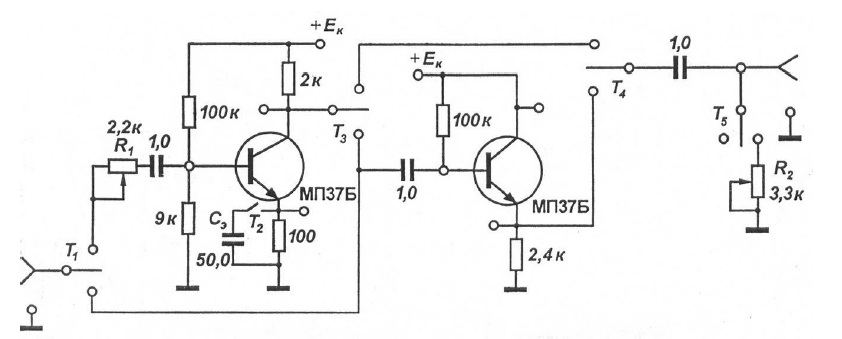
\includegraphics[width=\linewidth]{fig/fig7}
	\caption{}
	\label{fig:7}
\end{figure}

\section{Описание лабораторной установки}
Все элементы исследуемых каскадов установлены под верхней панелью макета и соединены между собой в соответствии со схемой (см.рис.\ref{fig:7}).

Питание выходных цепей каскадов производится от встроенного в макет источника напряжения $E_K=9B$.

Для установки начальной рабочей точки во входную цепь подано напряжение смещения. В схеме с ОЭ смещение задается делителем в цепи базы; в схеме с ОК - определяется фиксированным током базы через резистор в цепи базы.

Резистор в цепи эмиттера в схеме с ОЭ служит для температурной стабилизации рабочей точки, за счет возникающей при включении резистора отрицательной обратной связи по постоянному току. Для частот сигнала этот резистор "закорачивается" шунтирующим его конденсатором большой емкости $C_{\text{Э}}$.

Резистор в цепи коллектора в схеме с ОЭ и резистор в цепи эмиттера в схеме с ОК являются сопротивлениями нагрузки. Потенциометр $R_1$ служит для измерения входного сопротивления
каскада с ОЭ, $R_2$ - внешняя нагрузка.

Соединения между каскадами, подключение внешней нагрузки $R_2$, а также подключения емкости CЭ осуществляются с помощью соответствующих тумблеров $T_1$, $T_2$, $T_3$, $T_4$ и $T_5$ на верхней панели.

Генератор стандартных сигналов и вольтметр для измерения амплитуды входного сигнала подключаются к разъему на левой боковой стенке макета. Осциллограф и вольтметр для измерения амплитуды сигнала на выходе усилителя подключаются к разъему на правой боковой стенке.
\end{document}

